\section{Simulation of gamma-ray signals from dark matter subhalos}
\label{app:sim-ps}

In this appendix we provide details about the simulation of gamma-ray signal from DM subhalos.
Eq.~(\ref{eq:pDM}) describes the probability of observing a DM subhalo 
given a DM model.
This equation includes three terms that need to be estimated through simulations: 
the number density $n(\phi_\textrm{DM})$ of DM subhalos as a function of expected flux (section~\ref{sec:DM_model}), the probability $p_\textrm{DM}(\alpha,\beta|\phi_\textrm{DM};\btheta_\textrm{DM})$  of observing a source with the log-parabola spectrum parameters $(\alpha,\,\beta)$ given a DM model, which we obtain by computing and fitting simulations of DM point sources, and the efficiency $\varepsilon_\textrm{eff}(\phi_\textrm{DM})$ of the detection of a source, which we obtain from the same set of simulations by identifying the fraction of sources which can be detected by \Fermi-LAT.  
We now describe how the DM distribution conditioned on the gamma-ray flux is derived and how we estimate the detection efficiency for DM subhalos.

We compute the DM distribution  conditioned on the gamma-ray flux, through realistic photon-counts simulations of DM point sources. 
We decompose the gamma-ray sky into two  components: a diffuse emission component (constituted by the diffuse Galactic emission and an isotropic background) and the signal from the DM point sources. 
We model the diffuse Galactic emission using the \verb|gll_iem_v7| template provided by the \Fermi-LAT collaboration as well as the corresponding isotropic background model.
We integrate eq.~(\ref{eq:DM_spec}) in 16 logarithmic energy bins between 100 MeV and 1 TeV to obtain the theoretical energy spectrum in units of the photon flux per energy bin.
We specify the spectral energy distribution (SED), $dN_\gamma/dE$, using the recent estimations from CosmiXs \cite{2024JCAP...03..035A}.

Furthermore, we notice that the J-factor and annihilation cross-section term factor out of the integral into an overall constant that ultimately defines the total flux normalization: 
\begin{equation}
   \Phi_i = A \int_{E_{min, i}}^{E_{max,i} }\frac{dN_\gamma}{dE}dE \,.
\end{equation}

For this reason, once we fix the SED for a specific DM annihilation channel and mass, the energy spectrum $\phi(E)$ is defined except for an energy-independent normalization term. 
By fixing the overall flux normalization, we obtain the expected gamma-ray flux due to a specific DM source. 
Experimental uncertainties in the reconstruction of energy and direction of gamma rays induce a spread in the distribution of photons associated with a point source.
We simulate sources by convolving with the \Fermi-LAT point spread function (PSF) and exposure
using {\Fermi} Science Tools (fermitools) version 2.2.0\footnote{\url{https://github.com/fermi-lat/Fermitools-conda/wiki}}.

In table \ref{tab:settings} we summarize the analysis settings, which are similar to the standard event selection cuts used in the construction of gamma-ray source catalogs. 
Likewise, we convolve the diffuse Galactic foreground and isotropic emission with the PSF and exposure to obtain the diffuse foreground emission.
For each simulation, we add the emission from 10,000 DM sources randomly and isotropically distributed in the sky together with the foreground emission. We chose this number of sources to roughly match the number of resolved sources in the 4FGL catalog and to have sufficient statistics for the DM sources, while avoiding excessively demanding simulations. We thus obtain a map for the expected photon counts due to a DM population with a specific mass, annihilation channel, and a common flux.

\begin{table}[t]
\centering
\begin{tabular}{ | l| l|  }
\hline
Healpix order & 8\\ 
Weeks & $9-795$\\ 
Emin & 100 MeV\\
Emax & 1 TeV\\
Instrument Response Functions (IRFs) & {\tt P8R3\_SOURCE\_V3} \\
EVCLASS & 128 (Source)\\ 
EVTYPE & 3 (Front+Back)\\
ZMAX & $90^\circ$ under 1 GeV, $105^\circ$ otherwise\\
Galactic foreground model & \verb|gll_iem_v7.fits| \\
\hline
\end{tabular}
\caption{{\tt Fermi Science Tools} settings used for the 15-year data set analysis.}
\label{tab:settings}
\end{table}

We employ each simulation (associated with a specific total gamma-ray flux for the DM source) to estimate $p_\textrm{DM}(\alpha,\beta|\phi_\textrm{DM};\btheta_\textrm{DM})$ as follows.
First, we perform a Poisson realization of the expected photon counts map.
Then we proceed with fitting the energy spectrum of each source with a log parabola function (with a fixed spatial position), yielding the DM distribution conditioned on the flux.
Finally, we estimate the detection efficiency $\varepsilon_\textrm{eff}(\phi_\textrm{DM})$ by studying the TS of the DM sources for a given map. We define the TS of a source by comparing the overall likelihood with and without the target source. We define the TS as:
\begin{equation}
TS = -2\ln\left(\frac{\mathcal{L}}{\mathcal{L}_0}\right),
\end{equation}
where $\mathcal{L}$ is the likelihood of the best fit model including the source, and $\mathcal{L}_0$ is the likelihood of the model without the source. 
If the TS of a source is larger than 25 we include that source to a database of resolved sources, for which the SED fit parameters are reliable and can be used for the estimation of $p_\textrm{DM}(\alpha,\beta|\phi_\textrm{DM};\btheta_\textrm{DM})$. Else, we discard the source as a low TS source which would not be measured by the {\Fermi} LAT.

The detection efficiency $\varepsilon_\textrm{eff}(\phi_\textrm{DM})$ of the {\Fermi} LAT to a DM source with a specific flux and SED is then defined as the ratio between the number of detected sources and the overall number of sources included in the simulation: 
\be
\varepsilon_\textrm{eff} = \frac{N_\textrm{sources}(TS>25)}{N_\textrm{sources}^\textrm{tot}}.
\ee

\begin{figure}
    \centering
    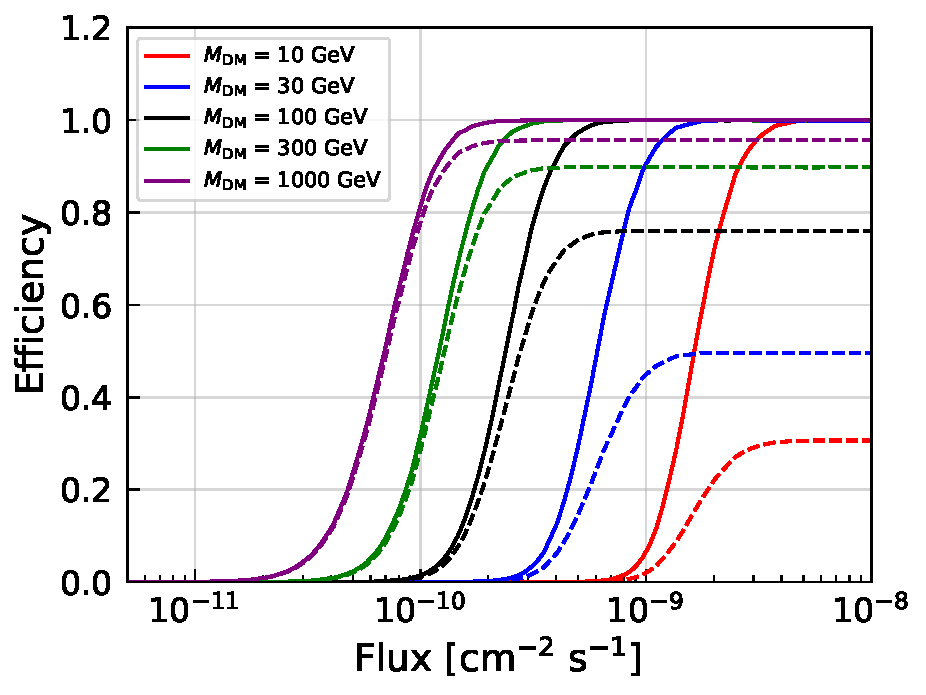
\includegraphics[width=0.5\linewidth]{img/efficiency/efficiency_bb_corrected.pdf}
    \caption{Detection efficiency for the $b\overline{b}$ annihilation channel simulations. \new{Solid lines denote the baseline efficiency used in the analysis, derived from simulations that disregard known 4FGL sources. Dashed lines illustrate a conservatively corrected efficiency, representing a worst-case scenario where a disk around each 4FGL source is masked to estimate the maximum potential degradation caused by their inclusion.}}

    \label{fig:efficiency}
\end{figure}

In order to avoid biasing the estimation of the DM distribution due to a low number of detectable sources or due to a very specific realization of the sky, we perform additional simulations of the gamma-ray sky until we detect a total of at least 20,000 DM sources or until 1,000 simulations have been performed. 
Once we have built a dataset of measurements for the energy spectrum of DM sources, we estimate the probability density function $p_{DM}(\alpha, \beta|\phi_{DM})$ by employing KDE, in analogy with what we did in section~\ref{sec:stat-model} for the astrophysical sources.

Due to the high number of DM sources, and the large number of simulations, we cannot employ the full detection and characterization pipeline which is usually adopted by the \Fermi-LAT collaboration.
We exploit the additional information available to us from simulations to perform a simplified analysis pipeline. 
The true energy spectrum of each DM source is fixed (and known) in our simulations, and so are the foreground components. The positions of the DM sources are known as well, and the sources are all point-like sources. For these reasons, we make the following assumptions in our analysis:
\begin{itemize}
    \item We assume that the energy spectrum of each background source (i.e. any source different from the one we are fitting) is known and fixed to the theoretical one (while in general they are jointly optimized together with the target of the fit);
    \item We fix the diffuse Galactic and the isotropic background components;
    \item We assume that the localization of the source is known (which in this case is true, but not in the case of source detection on real data);
    \item We assume that there are no low TS background sources, as we know exactly what we put inside our simulation.
    \item \new{We assume that contributions from known 4FGL sources are negligible when estimating the DM distribution. While these bright sources can reduce detection efficiency and should ideally be modeled jointly, we estimate the maximum degradation by masking a disk around each 4FGL source. 
    This mask corresponds to the 68\% containment angle of the PSF at the peak energy ($E_{peak}$) of the DM spectrum for each considered mass. Because the peak of the DM energy spectrum increases with the DM mass, the detection efficiency is affected more significantly at lower DM masses, as displayed in figure~\ref{fig:efficiency}. Specifically, for $\mdm$ $\geq$100 GeV, the narrower PSF results in a masked sky fraction of 20\% or less, deteriorating the bounds by approximately 15\%. 
    Conversely, for lower masses ($\mdm = 10 - 30$ GeV), the broader PSF yields a masked fraction of $50 - 70$\%, leading to a $35 - 60$\% degradation of the bounds. 
    Except for the $\mdm$ = 10 GeV case, this degradation remains within the bootstrap uncertainty band derived for the unmasked analysis. Nonetheless, we conservatively adjust the 95\% upper confidence level in figure~\ref{fig:bounds-bb} to account for these systematic effects.}
\end{itemize}

By making these assumptions, we fit each DM source individually, regardless of the others.

To perform a maximum likelihood estimation fit of the DM energy spectrum for each source, we define the likelihood as follows:
\begin{equation}
    \mathcal{L} = \prod_{e=1}^{N_{bin}} \prod_{j \, \in \, \textrm{disc}_e}  
    \mathcal{P}(k_{e,j}, \lambda_{e,j}(\bx)).
\end{equation}
Specifically, for each energy bin, we identify a disc around the source corresponding to the 95\% containment angle of the PSF with a minimal angle of $0.5^\circ$ and a maximal angle of $5^\circ$.
This ensures high enough statistics for the high-energy bins, and reduces the background noise for the low-energy bins, while leaving the intermediate-energy bins unaffected. 


For each pixel of the disc, we compare the photon counts $k_{ij}$ with the estimated photon counts $\lambda_{ij}(\bx)$ using the Poisson likelihood. The estimated photon counts are a sum of the Galactic foreground in the disc, the isotropic background, the emission of the other background (fixed) DM sources and the photon counts coming from the target source:
\begin{equation}
    \lambda(\bx) = \lambda_{gal} + \lambda_{iso} + \lambda_{S \neq S_i} + \lambda_{S_i}(\bx).
\end{equation}
Specifically, for a source $i$ and pixels $j$:
\begin{equation}
    \lambda_{S_i, e,j} = \left[\int_{E_{min}^e}^{E_{max}^e} \phi_{0,i}\frac{E}{E_0}^{-\alpha_i - \beta_i\log(E/E_0)} dE\right] \cdot \mathrm{PSF_{i,j}^e} \cdot \mathrm{exposure_{j}^e} \cdot \frac{4\pi}{12 N_\mathrm{side}^2}.
    \label{eq:lambda}
\end{equation}
We repeat the fitting procedure for each DM source, at a fixed total flux, and we build the DM distribution $p_{DM}(\alpha, \beta|\phi)\equiv p_{DM}^{KDE}(\alpha, \beta|\phi)$ through the KDE.

